\section{Streams}


\subsection{Konzept}

\begin{frame}{Datenfluss}
	\begin{itemize}
		\item Container dienen zur Speicherung von Daten
		\item Streams dienen zum Versenden oder Empfangen von Daten\\
		      $\implies$ Datenfluss
		\item Meist entweder nur source (read-only) oder nur sink (write-only)
		\item Puffern von Datensequenzen vor der Übertragung
		\item InputIterator (read-only, forward-only) für sources
		\item OutputIterator (write-only, forward-only) für sinks
	\end{itemize}
\end{frame}


\subsection{STL-Streams}

\begin{frame}[fragile]{Grundlegendes}
	\begin{itemize}
		\item STL-Streams sind hauptsächlich character-Streams
		\item Die eigentliche Übertragungs-Funktionalität steckt im Puffer!
		\item dienen dem Vereinfachten Zugriff auf Puffer
		\item Zustands-behaftet z.B. für Eingabe mit fester Breite (\verb|setw|)
	\end{itemize}
\end{frame}


\subsection{locales}

\begin{frame}{Locales}
	Unterschiedliche Konventionen in verschiedenen Ländern:
	
	\vspace{1em}
	
	\begin{tabular}{c|c|c}
		\textbf{USA}	&	\textbf{France}	&	\textbf{Deutschland}	\\
		\hline
		$3,042.12$		&	$3\;042,12$		&	$3\;042,12$				\\
		2:00 pm			&	14~h~05			&	14:00					\\
		June 22, 1996	&	22 juin 1996	&	22. Juni 1996			\\
	\end{tabular}
	
	\pause
	\vspace{0.5em}
	
	\begin{block}{Locale}
		Beschreibt Regions-spezifische Aspekte des UI, z.B.
		\begin{itemize}
			\item Zahlenformatierung
			\item Minuskel/Majuskel-Konversion
			\item Währung
			\item lexikographische Sortierung
			\item \dots
		\end{itemize}
	\end{block}
\end{frame}

\begin{frame}[fragile]{Locales in C++}
	\alert{ An sich eigenes Thema! }
	
	\pause
	\vspace{2em}
	
	\begin{lstlisting}[escapechar=\$]
		#include <locale>
		
		char const* const locale_name = "...";	// implementation-defined!
		std::locale loc(locale_name);
		
		char Ue = std::toupper('$ü$', loc);	// Ue == '$Ü$'
		char foo = std::toupper('$ß$', loc);	// foo == '$ß$' [sic!]
	\end{lstlisting}
	
	\vspace{1em}
	Meist aber indirekte Verwendung, z.B. über Streams.
\end{frame}


\subsection{base classes}

\begin{frame}{class hierarchy}
	\includegraphics[width=\textwidth]{images/streams-class-hierarchy}
\end{frame}

\begin{frame}{\texttt{std::ios\_base}, Standard 27.4.2}
	Für Anwender tendenziell uninteressant!
	
	Hauptsächlicher Inhalt:
	\begin{itemize}
		\item Formattierungs-Status (z.B. \texttt{std::ios\_base::width} $\leftarrow$ \texttt{setw})	\\
		(üblicherweise mittels stream manipulators)
		\item Einführung von Konstanten und Typen
		\item private storage
		\item callback registration
	\end{itemize}
	
	\footnotesize
	\begin{block}{Konstanten des Fehler-Zustands}
		% hack is quicker hacked than nice things are nicely done
		\begin{tabular}{ll}
			\texttt{0 == std::ios\_base::goodbit}	&	kein Fehler	\\
			\texttt{std::ios\_base::badbit}			&	\enquote{unheilbarer} Fehler	\\
			\texttt{std::ios\_base::failbit}		&	I/O Fehler (Formattierung oder Extraktion)	\\
			\texttt{std::ios\_base::eofbit}			&	Input hat das Dateiende erreicht (end-of-file)	\\
		\end{tabular}
	\end{block}
\end{frame}

\begin{frame}[fragile]{\texttt{std::basic\_ios} template}
	Hauptaufgabe: Management eines Puffers (\texttt{basic\_streambuf*})
	
	\vspace{2em}
	
	\begin{block}{Introducing: basic\_ios, Standard 27.4.4}
		\begin{lstlisting}
			template
			<
			    typename T_Char,
			    typename T_CharTraits = std::char_traits < T_Char >
			>
			class basic_ios;
		\end{lstlisting}
		
		\vspace{1em}
		
		\begin{description}[leftmargin=5em]
			\item[\texttt{T\_Char}] der zugrunde liegende Block-/Character-Datentyp
			\item[\texttt{T\_CharTraits}] \enquote{String}-Operationen und Eigenschaften von \texttt{T\_Char}
		\end{description}
	\end{block}
\end{frame}

\begin{frame}{\texttt{std::basic\_ios} Inhalt}
	Hauptsächlicher Inhalt:
	\begin{itemize}
		\item Fehler-Zustand
		\item \texttt{T\_CharT}-abhängiger Formattierungs-Status
		\item locale-Management
		\item Puffer-Ownership
	\end{itemize}
	
	\pause
	\vspace{2em}
	
	Fehler-Zustand lässt sich über diverse member functions abfragen und (zurück-)setzen.\\
	Wichtig: \texttt{eof}, \texttt{operator!}, \texttt{operator void*}
	
	\pause
	\vspace{2em}
	
	Zugrunde liegender Puffer lässt sich zur Laufzeit austauschen (\texttt{std::basic\_ios::rdbuf}).
\end{frame}

\begin{frame}{\texttt{std::basic\_streambuf}}
	Recht komplex!
	
	\pause
	\vspace{2em}
	
	Die ganze Funktionalität steckt in dieser abstrakten Klasse!
	
	Z.B.:
	\begin{itemize}
		\item Schreibe n character
		\item Lese n character
		\item \texttt{sync}, egtl. \enquote{flush} (Synchronisation mit dem Gerät)
	\end{itemize}
\end{frame}


\subsection{ostream}

\begin{frame}{\texttt{basic\_ostream} template}
	Hauptsächlicher Inhalt:
	\begin{itemize}
		\item formatted output, stream manipulator \enquote{interface}: \texttt{operator<<}
		\item unformatted output: \texttt{put}, \texttt{write}
		\item \texttt{flush}
		\item \texttt{sentry}-Klasse
	\end{itemize}
	
	\pause
	\vspace{2em}
	
	\begin{block}{sentry-Klasse}
		Kümmer Dich genau dann darum, wenn Du selbst eine \emph{formatted-output}-Funktion für einen Stream schreibt, die \emph{unformatted-output}-Funktionen nutzt (also nicht ausschließlich die standardmäßig vorhandenen \texttt{operator<<})!
	\end{block}
\end{frame}

\begin{frame}[fragile]{\texttt{basic\_ostream}: formatted output}
	\texttt{operator<<} standardmäßig schon definiert für:
	\begin{itemize}
		\item built-in data types (\texttt{short}, \texttt{int}, \texttt{bool}, \texttt{float} usw.)
		\item pointer (als \texttt{void const*})
		\item \texttt{std::basic\_streambuf}
		\item \texttt{std::string} (im Header \texttt{<string>})
		\item \texttt{char}, \texttt{char const*} und Abarten als globale Funktion
	\end{itemize}
	
	\pause
	\vspace{0.5em}
	
	\begin{block}{Verkettung von \texttt{operator<<}}
		Gibt \texttt{basic\_ostream < .... > \&} zurück, daher verketten möglich!
		\begin{lstlisting}
			/* 0. */  std::cout << 5  << "hallo";
			/* 1. */ (std::cout << 5) << "hallo";
			/* 2. */ std::ostream& rcout = std::cout << 5;
			         rcout << "hallo";
		\end{lstlisting}
	\end{block}
\end{frame}

\begin{frame}{stream manipulators}
	Schon bekannt:
	\begin{itemize}
		\item \texttt{std::endl}, \texttt{std::flush}
		\item \texttt{std::setw}, \texttt{std::setprecision}
	\end{itemize}
	
	\pause
	\vspace{2em}
	
	Finden sich in \texttt{<ios>}, \texttt{<ostream>} bzw. \texttt{<istream>} und in \texttt{<iomanip>}!
\end{frame}

\begin{frame}[fragile]{stream manips: Funktionsweise}
	\footnotesize
	die Manipulatoren
	\begin{itemize}
		\item beschreiben Funktionen (sind Funktionen $\implies$ function ptrs)
		\item werden mit \verb|operator<<| bzw. \verb|operator>>| an den Stream \enquote{übergeben}
		\item der Stream ruft die Funktion auf und übergibt sich selbst als Parameter
		\item die Manipulator-Funktion arbeitet auf dem Stream
	\end{itemize}
	
	\pause
	
	\begin{block}{Erläuterndes Beispiel}
		\begin{lstlisting}[basicstyle=\tiny, xleftmargin=3em]
			std::ostream& endl( std::ostream& p ) {
			    p.put( p.widen('\n') );
			    p.flush();
			    return p;
			}
			
			std::ostream& operator<< (std::ostream& p, Manipulator m) {
			    m(p);
			    return p;
			}
			
			std::cout << endl;
		\end{lstlisting}
	\end{block}
\end{frame}


\subsection{istream}

\begin{frame}{\texttt{basic\_istream} template}
	Hauptsächlicher Inhalt:
	\begin{itemize}
		\item formatted input, stream manipulator \enquote{interface}: \texttt{operator<<}
		\item unformatted input
		\item \texttt{sentry}-Klasse
	\end{itemize}
\end{frame}

\begin{frame}[fragile]{\texttt{basic\_istream}: formatted input}
	\texttt{operator<<} standardmäßig schon definiert für:
	\begin{itemize}
		\item built-in data types (\texttt{short}, \texttt{int}, \texttt{bool}, \texttt{float} usw.)
		\item pointer (als \texttt{void const*}
		\item \texttt{std::basic\_streambuf}
		\item \texttt{std::string} (im Header \texttt{<string>})
		\item \texttt{char} und Abarten als globale Funktion
		\item \alert{\texttt{char const*} und Abarten als globale Funktion, UNSAFE!}
	\end{itemize}
	Gibt \texttt{basic\_istream < .... > \&} zurück, daher verketten möglich! (\texttt{std::cin >> myInt >> myString;})
	
	\pause
	\vspace{1em}
	
	\begin{block}{Wichtig für formatted input}
		\texttt{operator>>} hört auf zu Lesen bei space-characters.
		space-characters sind locale-dependent! Zumeist aber mindestens:\\
		\verb|` '|, \verb|`\t'|, \verb|`\n'|, \verb|`v'|, \verb|`f'|, \verb|`\r'|
	\end{block}
\end{frame}

\begin{frame}[fragile]{Tipps zum formatted input}
	\footnotesize
	
	\begin{block}{\footnotesize Lesen bis EOF oder Fehler}
		\vspace{-0.5em}
		\begin{lstlisting}[basicstyle=\tiny]
			int i; double d;
			while(cin >> i >> d) {
			    // do something
			}
		\end{lstlisting}
		\vspace{-0.5em}
	\end{block}
	
	\pause
	
	\begin{block}{\footnotesize Lesen bis Trennzeichen (z.B. EOL)}
		\vspace{-0.5em}
		\begin{lstlisting}[basicstyle=\tiny]
			std::string target;
			while( getline(cin, target, '\n') ) {
			    // do something
			}
		\end{lstlisting}
		\vspace{-0.5em}
	\end{block}
	
	\pause
	
	\begin{block}{\footnotesize \enquote{Warten auf ENTER}}
		\vspace{-0.5em}
		\begin{lstlisting}[basicstyle=\tiny]
			// PITA!!
			std::cin.clear();                                            // Fehlerzustand aufheben
			if( 0 < std::cin.rdbuf()->in_avail() ) {                     // pruefe auf leeren Puffer
			    std::cin.ignore(                                         // leere Puffer
			        std::numeric_limits < std::streamsize > :: max(),
			        std::cin.widen('\n')
			    );
			}
			std::cin.get();                                              // Frage nach einem Zeichen
		\end{lstlisting}
		\vspace{-0.5em}
	\end{block}
\end{frame}


\subsection{konkrete Stream-Klassen}

\begin{frame}{\texttt{fstream}}
\end{frame}


\subsection{Standard-Streams}

\begin{frame}{Wohin gehen diese?}
	\begin{itemize}
		\item implementation-defined!
		\item meist: auf eine Konsole
		\item möglich: stream redirection / capture, z.B. Umleitung in Datei \texttt{myprog > myLog.log}
		\item C++ weiß noch nicht mal was von einer Tastatur!
	\end{itemize}
\end{frame}

\begin{frame}{\texttt{cin} und Konsorten}
	\begin{tabular}{cc}
		\textbf{Typ}	&	\textbf{Name}	& \textbf{Beschreibung}	\\
		\texttt{extern istream&}	&	\texttt{cin}	&	standard character input stream	\\
		\texttt{extern ostream&}	&	\texttt{cout}	&	standard character output stream	\\
		\texttt{extern ostream&}	&	\texttt{cerr}	&	standard character error stream	\\
		\texttt{extern ostream&}	&	\texttt{clog}	&	standard character log stream	\\
	\end{tabular}
	
	\vspace{2em}
	
	Das ganze gibt es noch als wide-character-Variante (anderes, weiteres Thema).
\end{frame}
